\documentclass[twoside]{book}

% Packages required by doxygen
\usepackage{fixltx2e}
\usepackage{calc}
\usepackage{doxygen}
\usepackage[export]{adjustbox} % also loads graphicx
\usepackage{graphicx}
\usepackage[utf8]{inputenc}
\usepackage{makeidx}
\usepackage{multicol}
\usepackage{multirow}
\PassOptionsToPackage{warn}{textcomp}
\usepackage{textcomp}
\usepackage[nointegrals]{wasysym}
\usepackage[table]{xcolor}

% Font selection
\usepackage[T1]{fontenc}
\usepackage[scaled=.90]{helvet}
\usepackage{courier}
\usepackage{amssymb}
\usepackage{sectsty}
\renewcommand{\familydefault}{\sfdefault}
\allsectionsfont{%
  \fontseries{bc}\selectfont%
  \color{darkgray}%
}
\renewcommand{\DoxyLabelFont}{%
  \fontseries{bc}\selectfont%
  \color{darkgray}%
}
\newcommand{\+}{\discretionary{\mbox{\scriptsize$\hookleftarrow$}}{}{}}

% Page & text layout
\usepackage{geometry}
\geometry{%
  a4paper,%
  top=2.5cm,%
  bottom=2.5cm,%
  left=2.5cm,%
  right=2.5cm%
}
\tolerance=750
\hfuzz=15pt
\hbadness=750
\setlength{\emergencystretch}{15pt}
\setlength{\parindent}{0cm}
\setlength{\parskip}{3ex plus 2ex minus 2ex}
\makeatletter
\renewcommand{\paragraph}{%
  \@startsection{paragraph}{4}{0ex}{-1.0ex}{1.0ex}{%
    \normalfont\normalsize\bfseries\SS@parafont%
  }%
}
\renewcommand{\subparagraph}{%
  \@startsection{subparagraph}{5}{0ex}{-1.0ex}{1.0ex}{%
    \normalfont\normalsize\bfseries\SS@subparafont%
  }%
}
\makeatother

% Headers & footers
\usepackage{fancyhdr}
\pagestyle{fancyplain}
\fancyhead[LE]{\fancyplain{}{\bfseries\thepage}}
\fancyhead[CE]{\fancyplain{}{}}
\fancyhead[RE]{\fancyplain{}{\bfseries\leftmark}}
\fancyhead[LO]{\fancyplain{}{\bfseries\rightmark}}
\fancyhead[CO]{\fancyplain{}{}}
\fancyhead[RO]{\fancyplain{}{\bfseries\thepage}}
\fancyfoot[LE]{\fancyplain{}{}}
\fancyfoot[CE]{\fancyplain{}{}}
\fancyfoot[RE]{\fancyplain{}{\bfseries\scriptsize Generated by Doxygen }}
\fancyfoot[LO]{\fancyplain{}{\bfseries\scriptsize Generated by Doxygen }}
\fancyfoot[CO]{\fancyplain{}{}}
\fancyfoot[RO]{\fancyplain{}{}}
\renewcommand{\footrulewidth}{0.4pt}
\renewcommand{\chaptermark}[1]{%
  \markboth{#1}{}%
}
\renewcommand{\sectionmark}[1]{%
  \markright{\thesection\ #1}%
}

% Indices & bibliography
\usepackage{natbib}
\usepackage[titles]{tocloft}
\setcounter{tocdepth}{3}
\setcounter{secnumdepth}{5}
\makeindex

% Hyperlinks (required, but should be loaded last)
\usepackage{ifpdf}
\ifpdf
  \usepackage[pdftex,pagebackref=true]{hyperref}
\else
  \usepackage[ps2pdf,pagebackref=true]{hyperref}
\fi
\hypersetup{%
  colorlinks=true,%
  linkcolor=blue,%
  citecolor=blue,%
  unicode%
}

% Custom commands
\newcommand{\clearemptydoublepage}{%
  \newpage{\pagestyle{empty}\cleardoublepage}%
}

\usepackage{caption}
\captionsetup{labelsep=space,justification=centering,font={bf},singlelinecheck=off,skip=4pt,position=top}

%===== C O N T E N T S =====

\begin{document}

% Titlepage & ToC
\hypersetup{pageanchor=false,
             bookmarksnumbered=true,
             pdfencoding=unicode
            }
\pagenumbering{roman}
\begin{titlepage}
\vspace*{7cm}
\begin{center}%
{\Large My Project }\\
\vspace*{1cm}
{\large Generated by Doxygen 1.8.11}\\
\end{center}
\end{titlepage}
\clearemptydoublepage
\tableofcontents
\clearemptydoublepage
\pagenumbering{arabic}
\hypersetup{pageanchor=true}

%--- Begin generated contents ---
\chapter{Hierarchical Index}
\section{Class Hierarchy}
This inheritance list is sorted roughly, but not completely, alphabetically\+:\begin{DoxyCompactList}
\item \contentsline{section}{auxiliary}{\pageref{classauxiliary}}{}
\item Drawing\+Area\begin{DoxyCompactList}
\item \contentsline{section}{My\+Area}{\pageref{classMyArea}}{}
\end{DoxyCompactList}
\item \contentsline{section}{Edge2d}{\pageref{classEdge2d}}{}
\item \contentsline{section}{Edge3d}{\pageref{classEdge3d}}{}
\item \contentsline{section}{file\+\_\+handle}{\pageref{classfile__handle}}{}
\item \contentsline{section}{object2d}{\pageref{classobject2d}}{}
\item \contentsline{section}{object3d}{\pageref{classobject3d}}{}
\item \contentsline{section}{projection}{\pageref{classprojection}}{}
\item \contentsline{section}{rev\+\_\+3dto2d}{\pageref{classrev__3dto2d}}{}
\item \contentsline{section}{Surface2d}{\pageref{classSurface2d}}{}
\item \contentsline{section}{Surface3d}{\pageref{classSurface3d}}{}
\item \contentsline{section}{Vertex2d}{\pageref{classVertex2d}}{}
\item \contentsline{section}{Vertex3d}{\pageref{classVertex3d}}{}
\item Window\begin{DoxyCompactList}
\item \contentsline{section}{Input2d\+Window}{\pageref{classInput2dWindow}}{}
\item \contentsline{section}{Input3d\+Window}{\pageref{classInput3dWindow}}{}
\item \contentsline{section}{Main\+Window}{\pageref{classMainWindow}}{}
\end{DoxyCompactList}
\end{DoxyCompactList}

\chapter{Class Index}
\section{Class List}
Here are the classes, structs, unions and interfaces with brief descriptions\+:\begin{DoxyCompactList}
\item\contentsline{section}{\hyperlink{classauxiliary}{auxiliary} }{\pageref{classauxiliary}}{}
\item\contentsline{section}{\hyperlink{classEdge2d}{Edge2d} }{\pageref{classEdge2d}}{}
\item\contentsline{section}{\hyperlink{classEdge3d}{Edge3d} }{\pageref{classEdge3d}}{}
\item\contentsline{section}{\hyperlink{classfile__handle}{file\+\_\+handle} }{\pageref{classfile__handle}}{}
\item\contentsline{section}{\hyperlink{classInput2dWindow}{Input2d\+Window} }{\pageref{classInput2dWindow}}{}
\item\contentsline{section}{\hyperlink{classInput3dWindow}{Input3d\+Window} }{\pageref{classInput3dWindow}}{}
\item\contentsline{section}{\hyperlink{classMainWindow}{Main\+Window} }{\pageref{classMainWindow}}{}
\item\contentsline{section}{\hyperlink{classMyArea}{My\+Area} }{\pageref{classMyArea}}{}
\item\contentsline{section}{\hyperlink{classobject2d}{object2d} }{\pageref{classobject2d}}{}
\item\contentsline{section}{\hyperlink{classobject3d}{object3d} }{\pageref{classobject3d}}{}
\item\contentsline{section}{\hyperlink{classprojection}{projection} }{\pageref{classprojection}}{}
\item\contentsline{section}{\hyperlink{classrev__3dto2d}{rev\+\_\+3dto2d} }{\pageref{classrev__3dto2d}}{}
\item\contentsline{section}{\hyperlink{classSurface2d}{Surface2d} }{\pageref{classSurface2d}}{}
\item\contentsline{section}{\hyperlink{classSurface3d}{Surface3d} }{\pageref{classSurface3d}}{}
\item\contentsline{section}{\hyperlink{classVertex2d}{Vertex2d} }{\pageref{classVertex2d}}{}
\item\contentsline{section}{\hyperlink{classVertex3d}{Vertex3d} }{\pageref{classVertex3d}}{}
\end{DoxyCompactList}

\chapter{Class Documentation}
\hypertarget{classauxiliary}{}\section{auxiliary Class Reference}
\label{classauxiliary}\index{auxiliary@{auxiliary}}
\subsection*{Public Member Functions}
\begin{DoxyCompactItemize}
\item 
void {\bfseries translate2d} (\hyperlink{classobject2d}{object2d} obj, vector$<$ double $>$ direction, double units)\hypertarget{classauxiliary_aad780e2b2b06f034da5940106573403e}{}\label{classauxiliary_aad780e2b2b06f034da5940106573403e}

\item 
void {\bfseries mirror2d} (\hyperlink{classobject2d}{object2d} obj, int direction)\hypertarget{classauxiliary_aad2eb20c84d63814e01851d13c2f391c}{}\label{classauxiliary_aad2eb20c84d63814e01851d13c2f391c}

\item 
void {\bfseries rotate2d} (\hyperlink{classobject2d}{object2d} obj, double radian)\hypertarget{classauxiliary_a677e3bb70dcd69ab7de7d90f435d06d3}{}\label{classauxiliary_a677e3bb70dcd69ab7de7d90f435d06d3}

\item 
void {\bfseries scale2d} (\hyperlink{classobject2d}{object2d} obj, double factor)\hypertarget{classauxiliary_a38835e6e55a85ca7b2f30dda9fb18ba2}{}\label{classauxiliary_a38835e6e55a85ca7b2f30dda9fb18ba2}

\item 
void {\bfseries shear2d} (\hyperlink{classobject2d}{object2d} obj, double factor, int direction)\hypertarget{classauxiliary_a802658ef07a2a749962de73d6e836f76}{}\label{classauxiliary_a802658ef07a2a749962de73d6e836f76}

\item 
void {\bfseries translate3d} (\hyperlink{classobject3d}{object3d} obj, vector$<$ double $>$ direction, double value)\hypertarget{classauxiliary_ad85868aa5b33d05ecf01887f537ae3c8}{}\label{classauxiliary_ad85868aa5b33d05ecf01887f537ae3c8}

\item 
void {\bfseries mirror3d} (\hyperlink{classobject3d}{object3d} obj, vector$<$ double $>$ plane)\hypertarget{classauxiliary_a2e70ba8ba76cf36bed9018c4276b368a}{}\label{classauxiliary_a2e70ba8ba76cf36bed9018c4276b368a}

\item 
void {\bfseries rotate3d} (\hyperlink{classobject3d}{object3d} obj, vector$<$ double $>$ direction, double radian)\hypertarget{classauxiliary_abce9263f052db4127cb6935a0a135b84}{}\label{classauxiliary_abce9263f052db4127cb6935a0a135b84}

\item 
void {\bfseries scale3d} (\hyperlink{classobject3d}{object3d} obj, double factor)\hypertarget{classauxiliary_a85ed61c481b9e7b16e85748f62ef3346}{}\label{classauxiliary_a85ed61c481b9e7b16e85748f62ef3346}

\end{DoxyCompactItemize}


The documentation for this class was generated from the following file\+:\begin{DoxyCompactItemize}
\item 
backend\+\_\+header.\+h\end{DoxyCompactItemize}

\hypertarget{classEdge2d}{}\section{Edge2d Class Reference}
\label{classEdge2d}\index{Edge2d@{Edge2d}}


Collaboration diagram for Edge2d\+:
\nopagebreak
\begin{figure}[H]
\begin{center}
\leavevmode
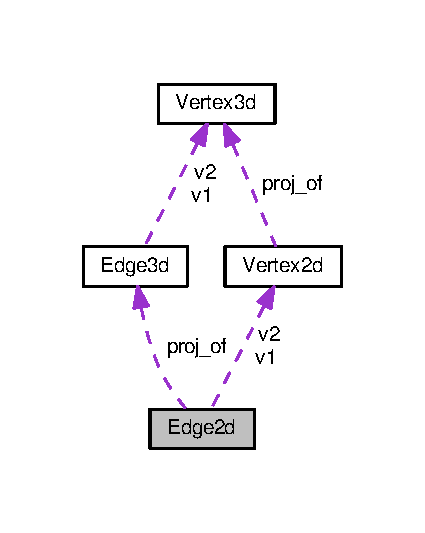
\includegraphics[width=204pt]{classEdge2d__coll__graph}
\end{center}
\end{figure}
\subsection*{Public Member Functions}
\begin{DoxyCompactItemize}
\item 
{\bfseries Edge2d} (\hyperlink{classVertex2d}{Vertex2d} v1\+\_\+c, \hyperlink{classVertex2d}{Vertex2d} v2\+\_\+c)\hypertarget{classEdge2d_a4cb7474a42b6736602cb7d4d86b6fab6}{}\label{classEdge2d_a4cb7474a42b6736602cb7d4d86b6fab6}

\item 
void {\bfseries translate} (vector$<$ double $>$ direction, double units)\hypertarget{classEdge2d_a6cffdd19332b65ab7777d220dc251308}{}\label{classEdge2d_a6cffdd19332b65ab7777d220dc251308}

\item 
void {\bfseries mirror} (int direction)\hypertarget{classEdge2d_aa03f4e523f21276047f28d2caba4dc69}{}\label{classEdge2d_aa03f4e523f21276047f28d2caba4dc69}

\item 
void {\bfseries rotate} (double radian)\hypertarget{classEdge2d_ad71932ada97c36f8179b139143d54a00}{}\label{classEdge2d_ad71932ada97c36f8179b139143d54a00}

\item 
void {\bfseries scale} (double factor)\hypertarget{classEdge2d_ae78424e5ef424ba038bbd4067598f93f}{}\label{classEdge2d_ae78424e5ef424ba038bbd4067598f93f}

\item 
void {\bfseries shear} (double factor, int direction)\hypertarget{classEdge2d_ab4a63d9d04470c857fcb268f31867595}{}\label{classEdge2d_ab4a63d9d04470c857fcb268f31867595}

\end{DoxyCompactItemize}
\subsection*{Public Attributes}
\begin{DoxyCompactItemize}
\item 
\hyperlink{classVertex2d}{Vertex2d} {\bfseries v1}\hypertarget{classEdge2d_a30f08d6392d2f0536687ac9f8eccb8f6}{}\label{classEdge2d_a30f08d6392d2f0536687ac9f8eccb8f6}

\item 
\hyperlink{classVertex2d}{Vertex2d} {\bfseries v2}\hypertarget{classEdge2d_aeb751a8cd6057d339b2389019487af07}{}\label{classEdge2d_aeb751a8cd6057d339b2389019487af07}

\item 
\hyperlink{classEdge3d}{Edge3d} {\bfseries proj\+\_\+of}\hypertarget{classEdge2d_adc9804b436746303fb3e883923eefdcf}{}\label{classEdge2d_adc9804b436746303fb3e883923eefdcf}

\item 
bool {\bfseries hidden}\hypertarget{classEdge2d_a2fefb205405c8af2d8e78c2cfabdc4c5}{}\label{classEdge2d_a2fefb205405c8af2d8e78c2cfabdc4c5}

\item 
string {\bfseries name}\hypertarget{classEdge2d_aebf763e48b3e401921dbfe3cc2aab879}{}\label{classEdge2d_aebf763e48b3e401921dbfe3cc2aab879}

\end{DoxyCompactItemize}


The documentation for this class was generated from the following file\+:\begin{DoxyCompactItemize}
\item 
backend\+\_\+header.\+h\end{DoxyCompactItemize}

\hypertarget{classEdge3d}{}\section{Edge3d Class Reference}
\label{classEdge3d}\index{Edge3d@{Edge3d}}


Collaboration diagram for Edge3d\+:
\nopagebreak
\begin{figure}[H]
\begin{center}
\leavevmode
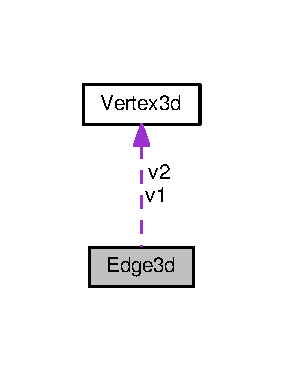
\includegraphics[width=136pt]{classEdge3d__coll__graph}
\end{center}
\end{figure}
\subsection*{Public Member Functions}
\begin{DoxyCompactItemize}
\item 
{\bfseries Edge3d} (\hyperlink{classVertex3d}{Vertex3d} v1\+\_\+c, \hyperlink{classVertex3d}{Vertex3d} v2\+\_\+c)\hypertarget{classEdge3d_aa3b092882195576dbd8279598eb9a25a}{}\label{classEdge3d_aa3b092882195576dbd8279598eb9a25a}

\item 
void {\bfseries translate} (vector$<$ double $>$ direction, double value)\hypertarget{classEdge3d_af1733ac8dae82923d56806ca15e2658a}{}\label{classEdge3d_af1733ac8dae82923d56806ca15e2658a}

\item 
void {\bfseries mirror} (vector$<$ double $>$ plane)\hypertarget{classEdge3d_a319cdf2988b30b8c04b42a984f44fbd8}{}\label{classEdge3d_a319cdf2988b30b8c04b42a984f44fbd8}

\item 
void {\bfseries rotate} (vector$<$ double $>$ direction, double radian)\hypertarget{classEdge3d_a74bc0bef90ff131c8639a47e97bd85c9}{}\label{classEdge3d_a74bc0bef90ff131c8639a47e97bd85c9}

\item 
void {\bfseries scale} (double factor)\hypertarget{classEdge3d_af27ff03f849dbeb3ac77a75ca9ba5594}{}\label{classEdge3d_af27ff03f849dbeb3ac77a75ca9ba5594}

\end{DoxyCompactItemize}
\subsection*{Public Attributes}
\begin{DoxyCompactItemize}
\item 
\hyperlink{classVertex3d}{Vertex3d} {\bfseries v1}\hypertarget{classEdge3d_a1feb11be268cbaf604da371ea3e13262}{}\label{classEdge3d_a1feb11be268cbaf604da371ea3e13262}

\item 
\hyperlink{classVertex3d}{Vertex3d} {\bfseries v2}\hypertarget{classEdge3d_ad821ed1fa2a5373926f9e54a8a11545e}{}\label{classEdge3d_ad821ed1fa2a5373926f9e54a8a11545e}

\item 
string {\bfseries name}\hypertarget{classEdge3d_a916daee4354abbf04b34792336eb7f0f}{}\label{classEdge3d_a916daee4354abbf04b34792336eb7f0f}

\end{DoxyCompactItemize}


The documentation for this class was generated from the following file\+:\begin{DoxyCompactItemize}
\item 
backend\+\_\+header.\+h\end{DoxyCompactItemize}

\hypertarget{classfile__handle}{}\section{file\+\_\+handle Class Reference}
\label{classfile__handle}\index{file\+\_\+handle@{file\+\_\+handle}}
\subsection*{Public Member Functions}
\begin{DoxyCompactItemize}
\item 
{\bfseries file\+\_\+handle} (string filename\+\_\+c)\hypertarget{classfile__handle_abe01c00c003b48cba1fec528a76131f4}{}\label{classfile__handle_abe01c00c003b48cba1fec528a76131f4}

\item 
\hyperlink{classobject2d}{object2d} {\bfseries input2d} ()\hypertarget{classfile__handle_a361d811f2c33e4031e0b31b1c79d8907}{}\label{classfile__handle_a361d811f2c33e4031e0b31b1c79d8907}

\item 
\hyperlink{classobject3d}{object3d} {\bfseries input3d} ()\hypertarget{classfile__handle_a237436534186b157c15066e2ad033afe}{}\label{classfile__handle_a237436534186b157c15066e2ad033afe}

\end{DoxyCompactItemize}
\subsection*{Public Attributes}
\begin{DoxyCompactItemize}
\item 
string {\bfseries filename}\hypertarget{classfile__handle_afe548bf4e2b6ac870b9dce7b979ca378}{}\label{classfile__handle_afe548bf4e2b6ac870b9dce7b979ca378}

\end{DoxyCompactItemize}


The documentation for this class was generated from the following file\+:\begin{DoxyCompactItemize}
\item 
file\+\_\+handle.\+h\end{DoxyCompactItemize}

\hypertarget{classInput2dWindow}{}\section{Input2d\+Window Class Reference}
\label{classInput2dWindow}\index{Input2d\+Window@{Input2d\+Window}}


Inheritance diagram for Input2d\+Window\+:
\nopagebreak
\begin{figure}[H]
\begin{center}
\leavevmode
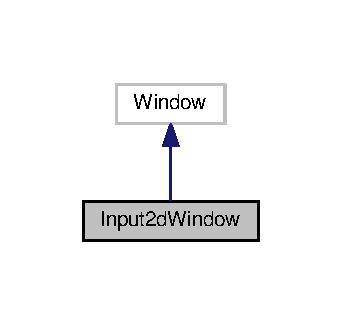
\includegraphics[width=164pt]{classInput2dWindow__inherit__graph}
\end{center}
\end{figure}


Collaboration diagram for Input2d\+Window\+:
\nopagebreak
\begin{figure}[H]
\begin{center}
\leavevmode
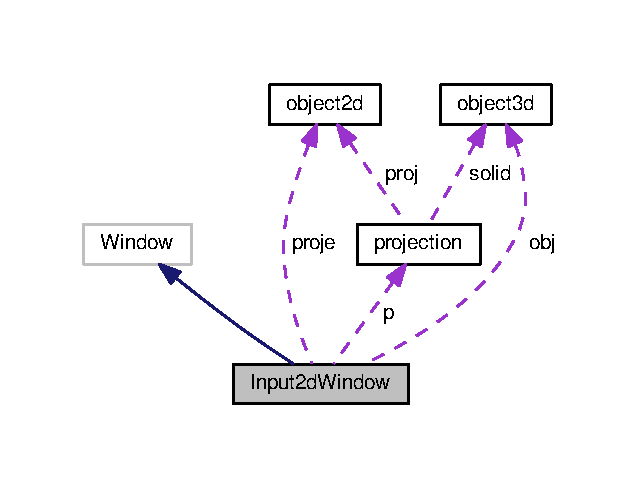
\includegraphics[width=307pt]{classInput2dWindow__coll__graph}
\end{center}
\end{figure}
\subsection*{Public Attributes}
\begin{DoxyCompactItemize}
\item 
string {\bfseries file\+\_\+xy}\hypertarget{classInput2dWindow_a8ed23971e947357b7116e051fb47f480}{}\label{classInput2dWindow_a8ed23971e947357b7116e051fb47f480}

\item 
string {\bfseries file\+\_\+yz}\hypertarget{classInput2dWindow_a46aac98c26f381b7db7601ddf2e555b8}{}\label{classInput2dWindow_a46aac98c26f381b7db7601ddf2e555b8}

\item 
string {\bfseries file\+\_\+zx}\hypertarget{classInput2dWindow_a892a6ec0b59229cad83a704145b0839d}{}\label{classInput2dWindow_a892a6ec0b59229cad83a704145b0839d}

\item 
\hyperlink{classobject3d}{object3d} {\bfseries obj}\hypertarget{classInput2dWindow_a5772c157faa4234226439c5480c36e7d}{}\label{classInput2dWindow_a5772c157faa4234226439c5480c36e7d}

\item 
vector$<$ double $>$ {\bfseries dir}\hypertarget{classInput2dWindow_ae05d43a211d36c34a7590f6d78484ef1}{}\label{classInput2dWindow_ae05d43a211d36c34a7590f6d78484ef1}

\item 
\hyperlink{classobject2d}{object2d} {\bfseries proje}\hypertarget{classInput2dWindow_a62904ea43cb0a6f4b709365de83c651f}{}\label{classInput2dWindow_a62904ea43cb0a6f4b709365de83c651f}

\item 
\hyperlink{classprojection}{projection} {\bfseries p}\hypertarget{classInput2dWindow_aa9e9f725b23c2dae7d90d148d2d79be1}{}\label{classInput2dWindow_aa9e9f725b23c2dae7d90d148d2d79be1}

\end{DoxyCompactItemize}
\subsection*{Protected Member Functions}
\begin{DoxyCompactItemize}
\item 
void {\bfseries on\+\_\+button\+\_\+submit} ()\hypertarget{classInput2dWindow_a095560d237009fea12e3ee651d7248b0}{}\label{classInput2dWindow_a095560d237009fea12e3ee651d7248b0}

\item 
void {\bfseries on\+\_\+button\+\_\+right} ()\hypertarget{classInput2dWindow_a55a69ce46e14b78cf1128ef25e899d93}{}\label{classInput2dWindow_a55a69ce46e14b78cf1128ef25e899d93}

\item 
void {\bfseries on\+\_\+button\+\_\+left} ()\hypertarget{classInput2dWindow_af0aeb7d0835fa4dc40b5c1ae39a495cb}{}\label{classInput2dWindow_af0aeb7d0835fa4dc40b5c1ae39a495cb}

\item 
void {\bfseries on\+\_\+button\+\_\+up} ()\hypertarget{classInput2dWindow_addc97f47f563b169b345279e460bc6d2}{}\label{classInput2dWindow_addc97f47f563b169b345279e460bc6d2}

\item 
void {\bfseries on\+\_\+button\+\_\+down} ()\hypertarget{classInput2dWindow_a60067e0c752da08a68c1ecef26808430}{}\label{classInput2dWindow_a60067e0c752da08a68c1ecef26808430}

\item 
void {\bfseries on\+\_\+button\+\_\+scale} ()\hypertarget{classInput2dWindow_aaf48d03bb2c28cbb2fa78075cee1a93a}{}\label{classInput2dWindow_aaf48d03bb2c28cbb2fa78075cee1a93a}

\item 
void {\bfseries on\+\_\+button\+\_\+trans} ()\hypertarget{classInput2dWindow_ac3c44172a5b85102df686e3c7c6ea5fd}{}\label{classInput2dWindow_ac3c44172a5b85102df686e3c7c6ea5fd}

\item 
bool {\bfseries on\+\_\+drawing} (const Cairo\+::\+Ref\+Ptr$<$ Cairo\+::\+Context $>$ \&cr)\hypertarget{classInput2dWindow_aa09359898d16c504732738e509534d27}{}\label{classInput2dWindow_aa09359898d16c504732738e509534d27}

\end{DoxyCompactItemize}
\subsection*{Protected Attributes}
\begin{DoxyCompactItemize}
\item 
Gtk\+::\+Drawing\+Area {\bfseries m\+\_\+area}\hypertarget{classInput2dWindow_a33f9df5ab0cb42c954384c4895167298}{}\label{classInput2dWindow_a33f9df5ab0cb42c954384c4895167298}

\item 
Gtk\+::\+Box {\bfseries m\+\_\+box}\hypertarget{classInput2dWindow_a52886df0c69c691f453cd55bbbe37484}{}\label{classInput2dWindow_a52886df0c69c691f453cd55bbbe37484}

\item 
Gtk\+::\+Frame {\bfseries m\+\_\+frame1}\hypertarget{classInput2dWindow_a30a13eb322c4a6995f3ca6fca7039caa}{}\label{classInput2dWindow_a30a13eb322c4a6995f3ca6fca7039caa}

\item 
Gtk\+::\+Frame {\bfseries m\+\_\+frame2}\hypertarget{classInput2dWindow_a133942a688c6c64bf5ca77800299a5d8}{}\label{classInput2dWindow_a133942a688c6c64bf5ca77800299a5d8}

\item 
Gtk\+::\+Frame {\bfseries m\+\_\+frame3}\hypertarget{classInput2dWindow_a9c8133ddbb2b6df871a6468e33aa2f40}{}\label{classInput2dWindow_a9c8133ddbb2b6df871a6468e33aa2f40}

\item 
Gtk\+::\+Grid {\bfseries m\+\_\+grid1}\hypertarget{classInput2dWindow_aa88d49ae5aca18f42394c43b7ca19061}{}\label{classInput2dWindow_aa88d49ae5aca18f42394c43b7ca19061}

\item 
Gtk\+::\+Grid {\bfseries m\+\_\+grid2}\hypertarget{classInput2dWindow_a5df326a3d367068f11307e2669df8b03}{}\label{classInput2dWindow_a5df326a3d367068f11307e2669df8b03}

\item 
Gtk\+::\+Button {\bfseries m\+\_\+button}\hypertarget{classInput2dWindow_a49e01c72961d67cee308cc996bdb980e}{}\label{classInput2dWindow_a49e01c72961d67cee308cc996bdb980e}

\item 
Gtk\+::\+Button {\bfseries m\+\_\+button\+\_\+r}\hypertarget{classInput2dWindow_ad06c022a8a99ee3f70d1c8c2a7af0b1a}{}\label{classInput2dWindow_ad06c022a8a99ee3f70d1c8c2a7af0b1a}

\item 
Gtk\+::\+Button {\bfseries m\+\_\+button\+\_\+l}\hypertarget{classInput2dWindow_aef1fa8fb41b55ee818f3f31e6e00a8b1}{}\label{classInput2dWindow_aef1fa8fb41b55ee818f3f31e6e00a8b1}

\item 
Gtk\+::\+Button {\bfseries m\+\_\+button\+\_\+u}\hypertarget{classInput2dWindow_ae8a9b15ff869d0c5bc498d610d1ce8ee}{}\label{classInput2dWindow_ae8a9b15ff869d0c5bc498d610d1ce8ee}

\item 
Gtk\+::\+Button {\bfseries m\+\_\+button\+\_\+d}\hypertarget{classInput2dWindow_ac3a0020ebede1ebad9243436fb0fb015}{}\label{classInput2dWindow_ac3a0020ebede1ebad9243436fb0fb015}

\item 
Gtk\+::\+Button {\bfseries m\+\_\+button\+\_\+scale}\hypertarget{classInput2dWindow_af7ff8c061d6954a1a60684b581c9b09a}{}\label{classInput2dWindow_af7ff8c061d6954a1a60684b581c9b09a}

\item 
Gtk\+::\+Button {\bfseries m\+\_\+button\+\_\+trans}\hypertarget{classInput2dWindow_a8099c28c32622131584cda737113b16e}{}\label{classInput2dWindow_a8099c28c32622131584cda737113b16e}

\item 
Gtk\+::\+Entry {\bfseries m\+\_\+file1}\hypertarget{classInput2dWindow_a1fb165a8575f3213004de2e2c06d7cc0}{}\label{classInput2dWindow_a1fb165a8575f3213004de2e2c06d7cc0}

\item 
Gtk\+::\+Entry {\bfseries m\+\_\+file2}\hypertarget{classInput2dWindow_afd1058d09326287b2e984308f73c1980}{}\label{classInput2dWindow_afd1058d09326287b2e984308f73c1980}

\item 
Gtk\+::\+Entry {\bfseries m\+\_\+file3}\hypertarget{classInput2dWindow_a4d6b681ed95c5af1d3e11074cba1c853}{}\label{classInput2dWindow_a4d6b681ed95c5af1d3e11074cba1c853}

\item 
Gtk\+::\+Entry {\bfseries m\+\_\+dir\+\_\+x}\hypertarget{classInput2dWindow_af4f60ca21bdb62581961f43a6b285538}{}\label{classInput2dWindow_af4f60ca21bdb62581961f43a6b285538}

\item 
Gtk\+::\+Entry {\bfseries m\+\_\+dir\+\_\+y}\hypertarget{classInput2dWindow_a70bd461b3757b4ffc246a8e04588710e}{}\label{classInput2dWindow_a70bd461b3757b4ffc246a8e04588710e}

\item 
Gtk\+::\+Entry {\bfseries m\+\_\+dir\+\_\+z}\hypertarget{classInput2dWindow_ad19551d7e3a340e8874f593736ca754e}{}\label{classInput2dWindow_ad19551d7e3a340e8874f593736ca754e}

\item 
Gtk\+::\+Entry {\bfseries m\+\_\+scale}\hypertarget{classInput2dWindow_a1aea837cc394544fcc67047e46c3383a}{}\label{classInput2dWindow_a1aea837cc394544fcc67047e46c3383a}

\item 
Gtk\+::\+Entry {\bfseries m\+\_\+trans\+\_\+x}\hypertarget{classInput2dWindow_abed706695b9f0acb22731918dde7de31}{}\label{classInput2dWindow_abed706695b9f0acb22731918dde7de31}

\item 
Gtk\+::\+Entry {\bfseries m\+\_\+trans\+\_\+y}\hypertarget{classInput2dWindow_a2b786777b7d43a86d76f1aa57b587f26}{}\label{classInput2dWindow_a2b786777b7d43a86d76f1aa57b587f26}

\item 
Gtk\+::\+Entry {\bfseries m\+\_\+trans\+\_\+z}\hypertarget{classInput2dWindow_a34e2c9b08ec2689612ae5e8a12abbe74}{}\label{classInput2dWindow_a34e2c9b08ec2689612ae5e8a12abbe74}

\item 
Gtk\+::\+Entry {\bfseries m\+\_\+trans\+\_\+amount}\hypertarget{classInput2dWindow_adfb4ddb2864e73385b1698d4e24401f6}{}\label{classInput2dWindow_adfb4ddb2864e73385b1698d4e24401f6}

\end{DoxyCompactItemize}


The documentation for this class was generated from the following files\+:\begin{DoxyCompactItemize}
\item 
display.\+h\item 
display.\+cpp\end{DoxyCompactItemize}

\hypertarget{classInput3dWindow}{}\section{Input3d\+Window Class Reference}
\label{classInput3dWindow}\index{Input3d\+Window@{Input3d\+Window}}


Inheritance diagram for Input3d\+Window\+:
\nopagebreak
\begin{figure}[H]
\begin{center}
\leavevmode
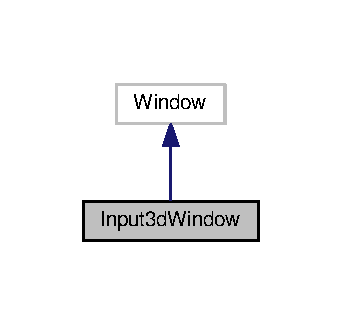
\includegraphics[width=164pt]{classInput3dWindow__inherit__graph}
\end{center}
\end{figure}


Collaboration diagram for Input3d\+Window\+:
\nopagebreak
\begin{figure}[H]
\begin{center}
\leavevmode
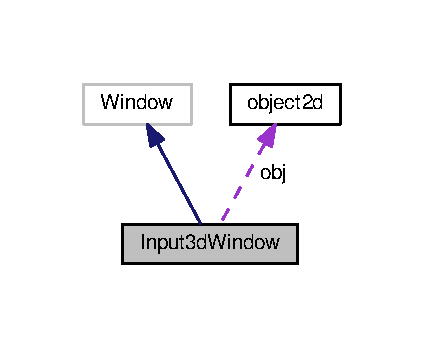
\includegraphics[width=204pt]{classInput3dWindow__coll__graph}
\end{center}
\end{figure}
\subsection*{Public Attributes}
\begin{DoxyCompactItemize}
\item 
\hyperlink{classobject2d}{object2d} {\bfseries obj}\hypertarget{classInput3dWindow_a2bd35358143316af1020cbccee0b9d7d}{}\label{classInput3dWindow_a2bd35358143316af1020cbccee0b9d7d}

\item 
string {\bfseries filename}\hypertarget{classInput3dWindow_a15f604279fd8d88c839c624925b45e10}{}\label{classInput3dWindow_a15f604279fd8d88c839c624925b45e10}

\end{DoxyCompactItemize}
\subsection*{Protected Member Functions}
\begin{DoxyCompactItemize}
\item 
void {\bfseries on\+\_\+button\+\_\+submit} ()\hypertarget{classInput3dWindow_a6620478dda7323a4e598dca1003ed3c9}{}\label{classInput3dWindow_a6620478dda7323a4e598dca1003ed3c9}

\item 
bool {\bfseries on\+\_\+drawing} (const Cairo\+::\+Ref\+Ptr$<$ Cairo\+::\+Context $>$ \&cr)\hypertarget{classInput3dWindow_abb61758284322bda2c9df6e343b396ae}{}\label{classInput3dWindow_abb61758284322bda2c9df6e343b396ae}

\end{DoxyCompactItemize}
\subsection*{Protected Attributes}
\begin{DoxyCompactItemize}
\item 
Gtk\+::\+Drawing\+Area {\bfseries m\+\_\+area}\hypertarget{classInput3dWindow_af4d22c728a235c13ef4a04709fcc3816}{}\label{classInput3dWindow_af4d22c728a235c13ef4a04709fcc3816}

\item 
Gtk\+::\+Box {\bfseries m\+\_\+box}\hypertarget{classInput3dWindow_a0b423e90d828a9ea2da836ae35daac37}{}\label{classInput3dWindow_a0b423e90d828a9ea2da836ae35daac37}

\item 
Gtk\+::\+Frame {\bfseries m\+\_\+frame1}\hypertarget{classInput3dWindow_a97b40510a0bd72ee8af7b97c3a8f0d76}{}\label{classInput3dWindow_a97b40510a0bd72ee8af7b97c3a8f0d76}

\item 
Gtk\+::\+Frame {\bfseries m\+\_\+frame2}\hypertarget{classInput3dWindow_a9b3c1a5603a9698638bbad2b9dfa270c}{}\label{classInput3dWindow_a9b3c1a5603a9698638bbad2b9dfa270c}

\item 
Gtk\+::\+Grid {\bfseries m\+\_\+grid}\hypertarget{classInput3dWindow_a00986d39a095c6d9fe231479965a4140}{}\label{classInput3dWindow_a00986d39a095c6d9fe231479965a4140}

\item 
Gtk\+::\+Button {\bfseries m\+\_\+button}\hypertarget{classInput3dWindow_a19b7bb9679cb057ddeed6709e0e80b22}{}\label{classInput3dWindow_a19b7bb9679cb057ddeed6709e0e80b22}

\item 
Gtk\+::\+Entry {\bfseries m\+\_\+filename}\hypertarget{classInput3dWindow_a238d6ef3aedc09602e24490a5eaa6ef7}{}\label{classInput3dWindow_a238d6ef3aedc09602e24490a5eaa6ef7}

\item 
Gtk\+::\+Entry {\bfseries m\+\_\+dir\+\_\+x}\hypertarget{classInput3dWindow_a12a865878cfbfc3bc4330f535dc17ce8}{}\label{classInput3dWindow_a12a865878cfbfc3bc4330f535dc17ce8}

\item 
Gtk\+::\+Entry {\bfseries m\+\_\+dir\+\_\+y}\hypertarget{classInput3dWindow_ab23381bd2cb6e05f80fad025a76aab29}{}\label{classInput3dWindow_ab23381bd2cb6e05f80fad025a76aab29}

\item 
Gtk\+::\+Entry {\bfseries m\+\_\+dir\+\_\+z}\hypertarget{classInput3dWindow_af2ba744e58fa7bad1ddbb98b5bfaad4f}{}\label{classInput3dWindow_af2ba744e58fa7bad1ddbb98b5bfaad4f}

\end{DoxyCompactItemize}


The documentation for this class was generated from the following files\+:\begin{DoxyCompactItemize}
\item 
display.\+h\item 
display.\+cpp\end{DoxyCompactItemize}

\hypertarget{classMainWindow}{}\section{Main\+Window Class Reference}
\label{classMainWindow}\index{Main\+Window@{Main\+Window}}


Inheritance diagram for Main\+Window\+:
\nopagebreak
\begin{figure}[H]
\begin{center}
\leavevmode
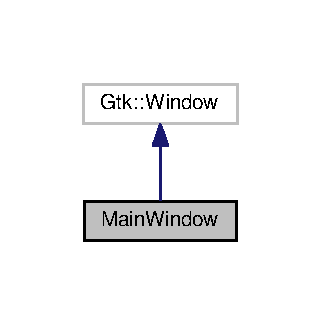
\includegraphics[width=154pt]{classMainWindow__inherit__graph}
\end{center}
\end{figure}


Collaboration diagram for Main\+Window\+:
\nopagebreak
\begin{figure}[H]
\begin{center}
\leavevmode
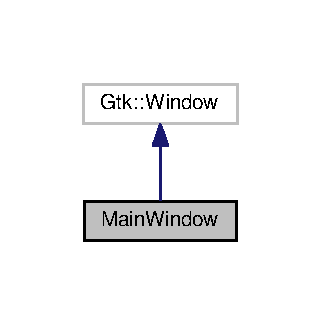
\includegraphics[width=154pt]{classMainWindow__coll__graph}
\end{center}
\end{figure}
\subsection*{Protected Member Functions}
\begin{DoxyCompactItemize}
\item 
void {\bfseries on\+\_\+button\+\_\+2d\+\_\+3d} ()\hypertarget{classMainWindow_a1259a864abd8c4397609e47fdfd57e91}{}\label{classMainWindow_a1259a864abd8c4397609e47fdfd57e91}

\item 
void {\bfseries on\+\_\+button\+\_\+3d\+\_\+2d} ()\hypertarget{classMainWindow_a50997436afe5e327ef6b8015767d4f59}{}\label{classMainWindow_a50997436afe5e327ef6b8015767d4f59}

\end{DoxyCompactItemize}
\subsection*{Protected Attributes}
\begin{DoxyCompactItemize}
\item 
Gtk\+::\+Box {\bfseries m\+\_\+box}\hypertarget{classMainWindow_ae9ef6a369c5adf6251cfcf8f6758b73d}{}\label{classMainWindow_ae9ef6a369c5adf6251cfcf8f6758b73d}

\item 
Gtk\+::\+Frame {\bfseries m\+\_\+frame}\hypertarget{classMainWindow_a8214cb1454a3434209091c9771205356}{}\label{classMainWindow_a8214cb1454a3434209091c9771205356}

\item 
Gtk\+::\+Grid {\bfseries m\+\_\+grid1}\hypertarget{classMainWindow_ad01fcce6ca67accc2b0cc8c3c512cbc2}{}\label{classMainWindow_ad01fcce6ca67accc2b0cc8c3c512cbc2}

\item 
Gtk\+::\+Grid {\bfseries m\+\_\+grid2}\hypertarget{classMainWindow_aeb023cb55e597ee1a0f0bf834944b127}{}\label{classMainWindow_aeb023cb55e597ee1a0f0bf834944b127}

\item 
Gtk\+::\+Button {\bfseries m\+\_\+button\+\_\+2d\+\_\+3d}\hypertarget{classMainWindow_a8746093c37f47022c2999c2f806464b0}{}\label{classMainWindow_a8746093c37f47022c2999c2f806464b0}

\item 
Gtk\+::\+Button {\bfseries m\+\_\+button\+\_\+3d\+\_\+2d}\hypertarget{classMainWindow_a0fb9c6d7aa1f9ac304ff16a16cc1650e}{}\label{classMainWindow_a0fb9c6d7aa1f9ac304ff16a16cc1650e}

\end{DoxyCompactItemize}


The documentation for this class was generated from the following files\+:\begin{DoxyCompactItemize}
\item 
display.\+h\item 
display.\+cpp\end{DoxyCompactItemize}

\hypertarget{classMyArea}{}\section{My\+Area Class Reference}
\label{classMyArea}\index{My\+Area@{My\+Area}}


Inheritance diagram for My\+Area\+:
\nopagebreak
\begin{figure}[H]
\begin{center}
\leavevmode
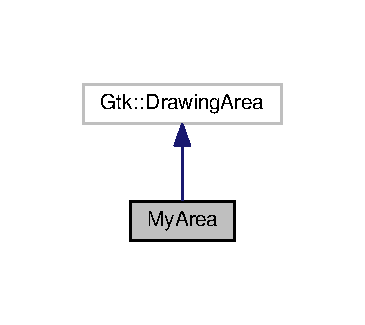
\includegraphics[width=175pt]{classMyArea__inherit__graph}
\end{center}
\end{figure}


Collaboration diagram for My\+Area\+:
\nopagebreak
\begin{figure}[H]
\begin{center}
\leavevmode
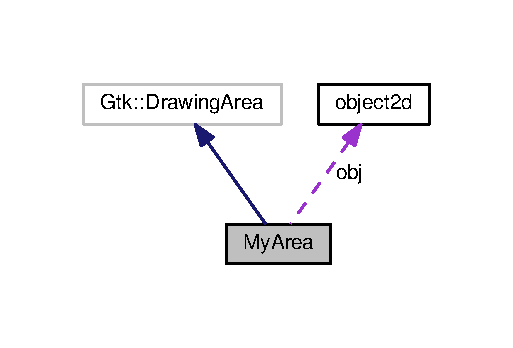
\includegraphics[width=246pt]{classMyArea__coll__graph}
\end{center}
\end{figure}
\subsection*{Public Attributes}
\begin{DoxyCompactItemize}
\item 
\hyperlink{classobject2d}{object2d} {\bfseries obj}\hypertarget{classMyArea_a08782571af573f253062bfc3e63e8567}{}\label{classMyArea_a08782571af573f253062bfc3e63e8567}

\end{DoxyCompactItemize}
\subsection*{Protected Member Functions}
\begin{DoxyCompactItemize}
\item 
bool {\bfseries on\+\_\+draw} (const Cairo\+::\+Ref\+Ptr$<$ Cairo\+::\+Context $>$ \&cr) override\hypertarget{classMyArea_af5d07988d7c9a6a623ba2fdd3332835b}{}\label{classMyArea_af5d07988d7c9a6a623ba2fdd3332835b}

\end{DoxyCompactItemize}


The documentation for this class was generated from the following file\+:\begin{DoxyCompactItemize}
\item 
display.\+h\end{DoxyCompactItemize}

\hypertarget{classobject2d}{}\section{object2d Class Reference}
\label{classobject2d}\index{object2d@{object2d}}
\subsection*{Public Member Functions}
\begin{DoxyCompactItemize}
\item 
void {\bfseries translate\+\_\+2d} (vector$<$ double $>$ direction, double units)\hypertarget{classobject2d_abf951e0ca5d840dd5879b466c99b6fd4}{}\label{classobject2d_abf951e0ca5d840dd5879b466c99b6fd4}

\item 
void {\bfseries mirror\+\_\+2d} (int direction)\hypertarget{classobject2d_a8b862ee5cca04cc04633061db32ddf5c}{}\label{classobject2d_a8b862ee5cca04cc04633061db32ddf5c}

\item 
void {\bfseries rotate\+\_\+2d} (double radian)\hypertarget{classobject2d_a3d03fc8df42b272c5c323c2b9c3446d7}{}\label{classobject2d_a3d03fc8df42b272c5c323c2b9c3446d7}

\item 
void {\bfseries scale\+\_\+2d} (double factor)\hypertarget{classobject2d_ae9f4b0b6b7394692bc15763349f62c3c}{}\label{classobject2d_ae9f4b0b6b7394692bc15763349f62c3c}

\item 
void {\bfseries shear\+\_\+2d} (double factor, int direction)\hypertarget{classobject2d_a95c7fb5d8298b20b96f66775617a141c}{}\label{classobject2d_a95c7fb5d8298b20b96f66775617a141c}

\end{DoxyCompactItemize}
\subsection*{Public Attributes}
\begin{DoxyCompactItemize}
\item 
vector$<$ \hyperlink{classVertex2d}{Vertex2d} $>$ {\bfseries vertices}\hypertarget{classobject2d_aefee0f3de7d38c69206bbb59835846d6}{}\label{classobject2d_aefee0f3de7d38c69206bbb59835846d6}

\item 
vector$<$ \hyperlink{classEdge2d}{Edge2d} $>$ {\bfseries edges}\hypertarget{classobject2d_ab9edc7a08e953d11902081c8f7148e5b}{}\label{classobject2d_ab9edc7a08e953d11902081c8f7148e5b}

\item 
vector$<$ \hyperlink{classSurface2d}{Surface2d} $>$ {\bfseries surfaces}\hypertarget{classobject2d_a7326212b9e3e600da4c391787d37e923}{}\label{classobject2d_a7326212b9e3e600da4c391787d37e923}

\item 
int {\bfseries num\+\_\+surface} = surfaces.\+size()\hypertarget{classobject2d_a79f784a84ef728b54ab87159b108641b}{}\label{classobject2d_a79f784a84ef728b54ab87159b108641b}

\end{DoxyCompactItemize}


The documentation for this class was generated from the following file\+:\begin{DoxyCompactItemize}
\item 
backend\+\_\+header.\+h\end{DoxyCompactItemize}

\hypertarget{classobject3d}{}\section{object3d Class Reference}
\label{classobject3d}\index{object3d@{object3d}}
\subsection*{Public Member Functions}
\begin{DoxyCompactItemize}
\item 
{\bfseries object3d} (vector$<$ \hyperlink{classVertex3d}{Vertex3d} $>$ vertices\+\_\+c, vector$<$ \hyperlink{classEdge3d}{Edge3d} $>$ edges\+\_\+c, vector$<$ \hyperlink{classSurface3d}{Surface3d} $>$ surfaces\+\_\+c)\hypertarget{classobject3d_a7ed942b90627e0dbf526ef9994e8c182}{}\label{classobject3d_a7ed942b90627e0dbf526ef9994e8c182}

\item 
void {\bfseries translate\+\_\+3d} (vector$<$ double $>$ direction, double value)\hypertarget{classobject3d_ae8b498e154077da23fe630d8c1ab5e99}{}\label{classobject3d_ae8b498e154077da23fe630d8c1ab5e99}

\item 
void {\bfseries mirror\+\_\+3d} (vector$<$ double $>$ plane)\hypertarget{classobject3d_ac09ec302c2e21ec0a51b8169347a8a1c}{}\label{classobject3d_ac09ec302c2e21ec0a51b8169347a8a1c}

\item 
void {\bfseries rotate\+\_\+3d} (vector$<$ double $>$ direction, double radian)\hypertarget{classobject3d_a86af8deddead81e682cdedcf1b3c3518}{}\label{classobject3d_a86af8deddead81e682cdedcf1b3c3518}

\item 
void {\bfseries scale\+\_\+3d} (double factor)\hypertarget{classobject3d_a5c889b19ad4dcd11c9bfa5e5c4042b00}{}\label{classobject3d_a5c889b19ad4dcd11c9bfa5e5c4042b00}

\end{DoxyCompactItemize}
\subsection*{Public Attributes}
\begin{DoxyCompactItemize}
\item 
vector$<$ \hyperlink{classVertex3d}{Vertex3d} $>$ {\bfseries vertices}\hypertarget{classobject3d_aa0d095ad6e321a6b3b7fc0d03305f9c0}{}\label{classobject3d_aa0d095ad6e321a6b3b7fc0d03305f9c0}

\item 
vector$<$ \hyperlink{classEdge3d}{Edge3d} $>$ {\bfseries edges}\hypertarget{classobject3d_a1faf7177578f0845f512712770c3f043}{}\label{classobject3d_a1faf7177578f0845f512712770c3f043}

\item 
vector$<$ \hyperlink{classSurface3d}{Surface3d} $>$ {\bfseries surfaces}\hypertarget{classobject3d_a91f9aa64272e9b66bd84842ca4a384a3}{}\label{classobject3d_a91f9aa64272e9b66bd84842ca4a384a3}

\end{DoxyCompactItemize}


The documentation for this class was generated from the following file\+:\begin{DoxyCompactItemize}
\item 
backend\+\_\+header.\+h\end{DoxyCompactItemize}

\hypertarget{classprojection}{}\section{projection Class Reference}
\label{classprojection}\index{projection@{projection}}


Collaboration diagram for projection\+:
\nopagebreak
\begin{figure}[H]
\begin{center}
\leavevmode
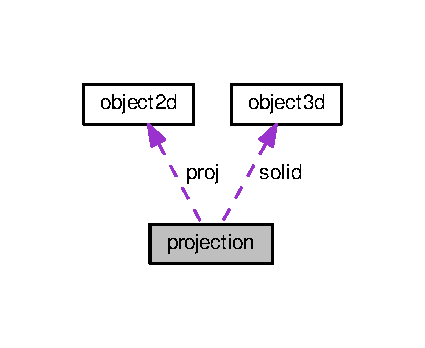
\includegraphics[width=204pt]{classprojection__coll__graph}
\end{center}
\end{figure}
\subsection*{Public Member Functions}
\begin{DoxyCompactItemize}
\item 
void {\bfseries project} ()\hypertarget{classprojection_a6a274f48a02d222f19eb058d6e54aacf}{}\label{classprojection_a6a274f48a02d222f19eb058d6e54aacf}

\item 
\hyperlink{classVertex2d}{Vertex2d} \hyperlink{classprojection_a538f0a0ffad6b4ab6280cfa5fb3b1fdb}{project\+\_\+v} (\hyperlink{classVertex3d}{Vertex3d} v)
\item 
\hyperlink{classEdge2d}{Edge2d} \hyperlink{classprojection_ae6b7e6a1773df79a6a3ca0f768699eb4}{project\+\_\+e} (\hyperlink{classEdge3d}{Edge3d} e)
\item 
\hyperlink{classSurface2d}{Surface2d} \hyperlink{classprojection_aa13c4e1c2676b918810e03f9b63d6a90}{project\+\_\+s} (\hyperlink{classSurface3d}{Surface3d} s)
\item 
double {\bfseries rotation\+\_\+angle} ()\hypertarget{classprojection_a32cfa1bcfa359224c9ec75144f77a6b4}{}\label{classprojection_a32cfa1bcfa359224c9ec75144f77a6b4}

\item 
void {\bfseries separate} ()\hypertarget{classprojection_ae2ba046447d1cf822f9f27c66e65db87}{}\label{classprojection_ae2ba046447d1cf822f9f27c66e65db87}

\item 
bool {\bfseries cut\+\_\+exist} (\hyperlink{classEdge2d}{Edge2d} e1, \hyperlink{classEdge2d}{Edge2d} e2)\hypertarget{classprojection_a13461be9eeda5f3abae6fe4f0917851a}{}\label{classprojection_a13461be9eeda5f3abae6fe4f0917851a}

\item 
\hyperlink{classVertex2d}{Vertex2d} {\bfseries find\+\_\+cut} (\hyperlink{classEdge2d}{Edge2d} e1, \hyperlink{classEdge2d}{Edge2d} e2)\hypertarget{classprojection_af38d729a67938a73090e348580ab4c0d}{}\label{classprojection_af38d729a67938a73090e348580ab4c0d}

\item 
bool {\bfseries locate\+\_\+cut} (\hyperlink{classVertex2d}{Vertex2d} v, \hyperlink{classEdge2d}{Edge2d} e)\hypertarget{classprojection_aa60b56e0c985de8508a88e42b9f139e9}{}\label{classprojection_aa60b56e0c985de8508a88e42b9f139e9}

\item 
void {\bfseries sort} (vector$<$ \hyperlink{classVertex2d}{Vertex2d} $>$ \&vec)\hypertarget{classprojection_a8732f1dd6eca7f8fe4a77fc29a8287d4}{}\label{classprojection_a8732f1dd6eca7f8fe4a77fc29a8287d4}

\item 
void {\bfseries create\+\_\+edges} (vector$<$ \hyperlink{classVertex2d}{Vertex2d} $>$ v, \hyperlink{classEdge2d}{Edge2d} e, vector$<$ \hyperlink{classEdge2d}{Edge2d} $>$ \&new\+\_\+edges)\hypertarget{classprojection_af4a7703ffcb0d8065161599fc0a53a0a}{}\label{classprojection_af4a7703ffcb0d8065161599fc0a53a0a}

\item 
void {\bfseries find\+\_\+coordinates} (\hyperlink{classEdge2d}{Edge2d} e, \hyperlink{classVertex2d}{Vertex2d} v, \hyperlink{classVertex3d}{Vertex3d} v\+\_\+3d)\hypertarget{classprojection_a5ed8afe4b9ddb6934964099ac8672d08}{}\label{classprojection_a5ed8afe4b9ddb6934964099ac8672d08}

\item 
void {\bfseries set\+\_\+bool} ()\hypertarget{classprojection_a309fd47b2fe6db11791c66b9109cb72f}{}\label{classprojection_a309fd47b2fe6db11791c66b9109cb72f}

\item 
bool {\bfseries check\+\_\+hidden} (\hyperlink{classEdge2d}{Edge2d} e)\hypertarget{classprojection_a9a39c01140c7f0a850a3399413f96d88}{}\label{classprojection_a9a39c01140c7f0a850a3399413f96d88}

\item 
bool {\bfseries hid\+\_\+by\+\_\+surf} (\hyperlink{classEdge2d}{Edge2d} e, \hyperlink{classSurface3d}{Surface3d} surface)\hypertarget{classprojection_a3f423bca7add8a35708563b4bdd9c91e}{}\label{classprojection_a3f423bca7add8a35708563b4bdd9c91e}

\item 
bool {\bfseries position\+\_\+fore} (\hyperlink{classVertex3d}{Vertex3d} v, \hyperlink{classSurface3d}{Surface3d} surface)\hypertarget{classprojection_adae33f33917c169cb26a30083fc5f362}{}\label{classprojection_adae33f33917c169cb26a30083fc5f362}

\item 
bool {\bfseries inside} (\hyperlink{classEdge2d}{Edge2d} e, \hyperlink{classSurface2d}{Surface2d} surface)\hypertarget{classprojection_a4800ad8659761e94c9361c8b0687716e}{}\label{classprojection_a4800ad8659761e94c9361c8b0687716e}

\item 
int \hyperlink{classprojection_a1472f7b496d0d3d12eed1445e970cde9}{position\+\_\+vert} (\hyperlink{classVertex2d}{Vertex2d} v, \hyperlink{classSurface2d}{Surface2d} surface)
\item 
bool {\bfseries on\+\_\+boundary} (\hyperlink{classVertex2d}{Vertex2d} v, \hyperlink{classSurface2d}{Surface2d} surface)\hypertarget{classprojection_a99d8290040437f3b902c27772176da5d}{}\label{classprojection_a99d8290040437f3b902c27772176da5d}

\item 
bool {\bfseries on\+\_\+edge} (\hyperlink{classVertex2d}{Vertex2d} v, \hyperlink{classEdge2d}{Edge2d} e)\hypertarget{classprojection_a816e0c9c71772b298d79a1f9acbab2d1}{}\label{classprojection_a816e0c9c71772b298d79a1f9acbab2d1}

\item 
int {\bfseries ray\+\_\+casting} (\hyperlink{classVertex2d}{Vertex2d} v, \hyperlink{classSurface2d}{Surface2d} surface)\hypertarget{classprojection_a66972c8979e1cb1429230f1759c313aa}{}\label{classprojection_a66972c8979e1cb1429230f1759c313aa}

\item 
int {\bfseries poly\+\_\+vertex} (\hyperlink{classVertex2d}{Vertex2d} v, \hyperlink{classSurface2d}{Surface2d} surface)\hypertarget{classprojection_a1850fe07fbd58a9b829dd65d931a73bf}{}\label{classprojection_a1850fe07fbd58a9b829dd65d931a73bf}

\item 
int {\bfseries coincident\+\_\+edge} (\hyperlink{classVertex2d}{Vertex2d} v, \hyperlink{classSurface2d}{Surface2d} surface)\hypertarget{classprojection_af35400b0243e982cbd9f9bee109de1ae}{}\label{classprojection_af35400b0243e982cbd9f9bee109de1ae}

\item 
int {\bfseries edge\+\_\+intersect} (\hyperlink{classVertex2d}{Vertex2d} v, \hyperlink{classSurface2d}{Surface2d} surface)\hypertarget{classprojection_a24d4d8db9c4b68ffd40f9eac528bbbb1}{}\label{classprojection_a24d4d8db9c4b68ffd40f9eac528bbbb1}

\item 
int {\bfseries check\+\_\+side\+\_\+vert} (\hyperlink{classVertex2d}{Vertex2d} v, \hyperlink{classSurface2d}{Surface2d} surface)\hypertarget{classprojection_afcfbb7569b94be5df14f252a1fd62774}{}\label{classprojection_afcfbb7569b94be5df14f252a1fd62774}

\item 
int {\bfseries check\+\_\+side\+\_\+edge} (\hyperlink{classEdge2d}{Edge2d} e, \hyperlink{classSurface2d}{Surface2d} surface)\hypertarget{classprojection_afe27008445491428359590360a821b84}{}\label{classprojection_afe27008445491428359590360a821b84}

\item 
int \hyperlink{classprojection_a09a4b15e0f9a7c687a7d417f4a51aa6e}{mid\+\_\+check} (\hyperlink{classVertex2d}{Vertex2d} v1, \hyperlink{classVertex2d}{Vertex2d} v2, \hyperlink{classSurface2d}{Surface2d} surface)
\item 
vector$<$ double $>$ {\bfseries cross} (vector$<$ double $>$ v1, vector$<$ double $>$ v2)\hypertarget{classprojection_a1bee2adde0b5145710546d870bb39303}{}\label{classprojection_a1bee2adde0b5145710546d870bb39303}

\end{DoxyCompactItemize}
\subsection*{Public Attributes}
\begin{DoxyCompactItemize}
\item 
\hyperlink{classobject3d}{object3d} {\bfseries solid}\hypertarget{classprojection_af10b79e4b507bc7242bcf875d86e3696}{}\label{classprojection_af10b79e4b507bc7242bcf875d86e3696}

\item 
\hyperlink{classobject2d}{object2d} {\bfseries proj}\hypertarget{classprojection_ae0d15d990e6573d75ff4d092fbd33679}{}\label{classprojection_ae0d15d990e6573d75ff4d092fbd33679}

\item 
vector$<$ double $>$ {\bfseries direction}\hypertarget{classprojection_a59d3d3752fef90fece215a4edae537b2}{}\label{classprojection_a59d3d3752fef90fece215a4edae537b2}

\end{DoxyCompactItemize}


\subsection{Member Function Documentation}
\index{projection@{projection}!mid\+\_\+check@{mid\+\_\+check}}
\index{mid\+\_\+check@{mid\+\_\+check}!projection@{projection}}
\subsubsection[{\texorpdfstring{mid\+\_\+check(\+Vertex2d v1, Vertex2d v2, Surface2d surface)}{mid_check(Vertex2d v1, Vertex2d v2, Surface2d surface)}}]{\setlength{\rightskip}{0pt plus 5cm}int projection\+::mid\+\_\+check (
\begin{DoxyParamCaption}
\item[{{\bf Vertex2d}}]{v1, }
\item[{{\bf Vertex2d}}]{v2, }
\item[{{\bf Surface2d}}]{surface}
\end{DoxyParamCaption}
)\hspace{0.3cm}{\ttfamily [inline]}}\hypertarget{classprojection_a09a4b15e0f9a7c687a7d417f4a51aa6e}{}\label{classprojection_a09a4b15e0f9a7c687a7d417f4a51aa6e}
returns the location of mid-\/point of v1 and v2\index{projection@{projection}!position\+\_\+vert@{position\+\_\+vert}}
\index{position\+\_\+vert@{position\+\_\+vert}!projection@{projection}}
\subsubsection[{\texorpdfstring{position\+\_\+vert(\+Vertex2d v, Surface2d surface)}{position_vert(Vertex2d v, Surface2d surface)}}]{\setlength{\rightskip}{0pt plus 5cm}int projection\+::position\+\_\+vert (
\begin{DoxyParamCaption}
\item[{{\bf Vertex2d}}]{v, }
\item[{{\bf Surface2d}}]{surface}
\end{DoxyParamCaption}
)\hspace{0.3cm}{\ttfamily [inline]}}\hypertarget{classprojection_a1472f7b496d0d3d12eed1445e970cde9}{}\label{classprojection_a1472f7b496d0d3d12eed1445e970cde9}
returns 0 if vert outside, 1 if inside, 2 if on the line\index{projection@{projection}!project\+\_\+e@{project\+\_\+e}}
\index{project\+\_\+e@{project\+\_\+e}!projection@{projection}}
\subsubsection[{\texorpdfstring{project\+\_\+e(\+Edge3d e)}{project_e(Edge3d e)}}]{\setlength{\rightskip}{0pt plus 5cm}{\bf Edge2d} projection\+::project\+\_\+e (
\begin{DoxyParamCaption}
\item[{{\bf Edge3d}}]{e}
\end{DoxyParamCaption}
)\hspace{0.3cm}{\ttfamily [inline]}}\hypertarget{classprojection_ae6b7e6a1773df79a6a3ca0f768699eb4}{}\label{classprojection_ae6b7e6a1773df79a6a3ca0f768699eb4}
\index{projection@{projection}!project\+\_\+s@{project\+\_\+s}}
\index{project\+\_\+s@{project\+\_\+s}!projection@{projection}}
\subsubsection[{\texorpdfstring{project\+\_\+s(\+Surface3d s)}{project_s(Surface3d s)}}]{\setlength{\rightskip}{0pt plus 5cm}{\bf Surface2d} projection\+::project\+\_\+s (
\begin{DoxyParamCaption}
\item[{{\bf Surface3d}}]{s}
\end{DoxyParamCaption}
)\hspace{0.3cm}{\ttfamily [inline]}}\hypertarget{classprojection_aa13c4e1c2676b918810e03f9b63d6a90}{}\label{classprojection_aa13c4e1c2676b918810e03f9b63d6a90}
\index{projection@{projection}!project\+\_\+v@{project\+\_\+v}}
\index{project\+\_\+v@{project\+\_\+v}!projection@{projection}}
\subsubsection[{\texorpdfstring{project\+\_\+v(\+Vertex3d v)}{project_v(Vertex3d v)}}]{\setlength{\rightskip}{0pt plus 5cm}{\bf Vertex2d} projection\+::project\+\_\+v (
\begin{DoxyParamCaption}
\item[{{\bf Vertex3d}}]{v}
\end{DoxyParamCaption}
)\hspace{0.3cm}{\ttfamily [inline]}}\hypertarget{classprojection_a538f0a0ffad6b4ab6280cfa5fb3b1fdb}{}\label{classprojection_a538f0a0ffad6b4ab6280cfa5fb3b1fdb}
Finds out the projection of a 3D vertex given a plane of projection by rotating the plane to coincide it with x-\/y plane.

The documentation for this class was generated from the following file\+:\begin{DoxyCompactItemize}
\item 
backend\+\_\+header.\+h\end{DoxyCompactItemize}

\hypertarget{classrev__3dto2d}{}\section{rev\+\_\+3dto2d Class Reference}
\label{classrev__3dto2d}\index{rev\+\_\+3dto2d@{rev\+\_\+3dto2d}}
\subsection*{Public Member Functions}
\begin{DoxyCompactItemize}
\item 
\hyperlink{classobject3d}{object3d} {\bfseries reconstruct3d} (\hyperlink{classobject2d}{object2d} obj1, \hyperlink{classobject2d}{object2d} obj2, \hyperlink{classobject2d}{object2d} obj3)\hypertarget{classrev__3dto2d_a30206736e5e95322b0dd301c596f32e1}{}\label{classrev__3dto2d_a30206736e5e95322b0dd301c596f32e1}

\item 
vector$<$ \hyperlink{classVertex3d}{Vertex3d} $>$ {\bfseries cor\+\_\+vertex} (\hyperlink{classobject2d}{object2d} obj1, \hyperlink{classobject2d}{object2d} obj2, \hyperlink{classobject2d}{object2d} obj3)\hypertarget{classrev__3dto2d_af83f643fa381b1f7689e77f00c55ea9a}{}\label{classrev__3dto2d_af83f643fa381b1f7689e77f00c55ea9a}

\item 
vector$<$ \hyperlink{classEdge3d}{Edge3d} $>$ {\bfseries cor\+\_\+edges} (\hyperlink{classobject2d}{object2d} obj1, \hyperlink{classobject2d}{object2d} obj2, \hyperlink{classobject2d}{object2d} obj3, vector$<$ \hyperlink{classVertex3d}{Vertex3d} $>$ vert)\hypertarget{classrev__3dto2d_a67089819dce28cd5e57ad691289590b2}{}\label{classrev__3dto2d_a67089819dce28cd5e57ad691289590b2}

\item 
int {\bfseries find} (vector$<$ \hyperlink{classVertex2d}{Vertex2d} $>$ set, \hyperlink{classVertex2d}{Vertex2d} s)\hypertarget{classrev__3dto2d_a64aff2d60828d570d02661dbd87eb78b}{}\label{classrev__3dto2d_a64aff2d60828d570d02661dbd87eb78b}

\item 
int {\bfseries find\+\_\+edge} (vector$<$ \hyperlink{classEdge2d}{Edge2d} $>$ set, \hyperlink{classEdge2d}{Edge2d} s)\hypertarget{classrev__3dto2d_a27a29f0711817222cae6d7f149051f48}{}\label{classrev__3dto2d_a27a29f0711817222cae6d7f149051f48}

\end{DoxyCompactItemize}


The documentation for this class was generated from the following file\+:\begin{DoxyCompactItemize}
\item 
backend\+\_\+header.\+h\end{DoxyCompactItemize}

\hypertarget{classSurface2d}{}\section{Surface2d Class Reference}
\label{classSurface2d}\index{Surface2d@{Surface2d}}
\subsection*{Public Member Functions}
\begin{DoxyCompactItemize}
\item 
{\bfseries Surface2d} (vector$<$ \hyperlink{classEdge2d}{Edge2d} $>$ edges\+\_\+c, int num\+\_\+edges\+\_\+c)\hypertarget{classSurface2d_ac22d9270baf7e6c489e9c49b7e4fba18}{}\label{classSurface2d_ac22d9270baf7e6c489e9c49b7e4fba18}

\item 
void {\bfseries translate} (vector$<$ double $>$ direction, double units)\hypertarget{classSurface2d_ae01681fb2a990db79d8ee715886c9742}{}\label{classSurface2d_ae01681fb2a990db79d8ee715886c9742}

\item 
void {\bfseries mirror} (int direction)\hypertarget{classSurface2d_ae827b73d9fb0a4d8085fd922cfd4cdc8}{}\label{classSurface2d_ae827b73d9fb0a4d8085fd922cfd4cdc8}

\item 
void {\bfseries rotate} (double radian)\hypertarget{classSurface2d_a1749d13ad536db0ebce644f4825585cf}{}\label{classSurface2d_a1749d13ad536db0ebce644f4825585cf}

\item 
void {\bfseries scale} (double factor)\hypertarget{classSurface2d_a18e70bf087f1676ddee54d38e0a142e2}{}\label{classSurface2d_a18e70bf087f1676ddee54d38e0a142e2}

\item 
void {\bfseries shear} (double factor, int direction)\hypertarget{classSurface2d_ac3727d4fbe2ab84a6d6332ac31514a18}{}\label{classSurface2d_ac3727d4fbe2ab84a6d6332ac31514a18}

\end{DoxyCompactItemize}
\subsection*{Public Attributes}
\begin{DoxyCompactItemize}
\item 
int {\bfseries num\+\_\+edges}\hypertarget{classSurface2d_abfd3a79363f04c26694262e17aa600e7}{}\label{classSurface2d_abfd3a79363f04c26694262e17aa600e7}

\item 
vector$<$ \hyperlink{classEdge2d}{Edge2d} $>$ {\bfseries edges}\hypertarget{classSurface2d_a05deea155e1b9b64fc02b922df17751c}{}\label{classSurface2d_a05deea155e1b9b64fc02b922df17751c}

\end{DoxyCompactItemize}


The documentation for this class was generated from the following file\+:\begin{DoxyCompactItemize}
\item 
backend\+\_\+header.\+h\end{DoxyCompactItemize}

\hypertarget{classSurface3d}{}\section{Surface3d Class Reference}
\label{classSurface3d}\index{Surface3d@{Surface3d}}
\subsection*{Public Member Functions}
\begin{DoxyCompactItemize}
\item 
{\bfseries Surface3d} (vector$<$ \hyperlink{classEdge3d}{Edge3d} $>$ edges\+\_\+c, int num\+\_\+edges\+\_\+c)\hypertarget{classSurface3d_a51aed86e66d73b012f0dbed3b437ec34}{}\label{classSurface3d_a51aed86e66d73b012f0dbed3b437ec34}

\item 
void {\bfseries translate} (vector$<$ double $>$ direction, double value)\hypertarget{classSurface3d_a72590543a4a60dedd9a932b50679b2ca}{}\label{classSurface3d_a72590543a4a60dedd9a932b50679b2ca}

\item 
void {\bfseries mirror} (vector$<$ double $>$ plane)\hypertarget{classSurface3d_a74ebcdd68b39cd0e59712164b4796b6c}{}\label{classSurface3d_a74ebcdd68b39cd0e59712164b4796b6c}

\item 
void {\bfseries rotate} (vector$<$ double $>$ direction, double radian)\hypertarget{classSurface3d_a625754b5b8f818559b343c4765e07ac3}{}\label{classSurface3d_a625754b5b8f818559b343c4765e07ac3}

\item 
void {\bfseries scale} (double factor)\hypertarget{classSurface3d_ac121aeaa939ad5a4dbf599d1b9d80e33}{}\label{classSurface3d_ac121aeaa939ad5a4dbf599d1b9d80e33}

\end{DoxyCompactItemize}
\subsection*{Public Attributes}
\begin{DoxyCompactItemize}
\item 
int {\bfseries num\+\_\+edges}\hypertarget{classSurface3d_a2e7b3c2dab341367ce52235b16756067}{}\label{classSurface3d_a2e7b3c2dab341367ce52235b16756067}

\item 
vector$<$ \hyperlink{classEdge3d}{Edge3d} $>$ {\bfseries edges}\hypertarget{classSurface3d_aad04d4bf228a38ec219f0fa1b5272ef8}{}\label{classSurface3d_aad04d4bf228a38ec219f0fa1b5272ef8}

\end{DoxyCompactItemize}


The documentation for this class was generated from the following file\+:\begin{DoxyCompactItemize}
\item 
backend\+\_\+header.\+h\end{DoxyCompactItemize}

\hypertarget{classVertex2d}{}\section{Vertex2d Class Reference}
\label{classVertex2d}\index{Vertex2d@{Vertex2d}}


Collaboration diagram for Vertex2d\+:
\nopagebreak
\begin{figure}[H]
\begin{center}
\leavevmode
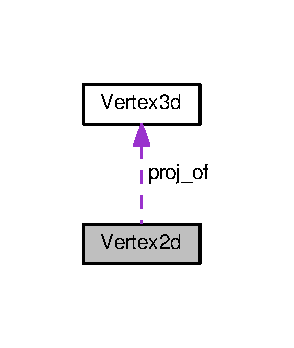
\includegraphics[width=141pt]{classVertex2d__coll__graph}
\end{center}
\end{figure}
\subsection*{Public Member Functions}
\begin{DoxyCompactItemize}
\item 
{\bfseries Vertex2d} (double first, double second, double third, string name\+\_\+c)\hypertarget{classVertex2d_afaf4e06289fec9a7a1703c506d7c9e4b}{}\label{classVertex2d_afaf4e06289fec9a7a1703c506d7c9e4b}

\item 
void {\bfseries translate} (vector$<$ double $>$ direction, double units)\hypertarget{classVertex2d_a2abdd1c5f5d7e3d694392d69f40985e8}{}\label{classVertex2d_a2abdd1c5f5d7e3d694392d69f40985e8}

\item 
void {\bfseries mirror} (int direction)\hypertarget{classVertex2d_a2cd4c427a421be1cd1a3c9e79eaa1740}{}\label{classVertex2d_a2cd4c427a421be1cd1a3c9e79eaa1740}

\item 
void {\bfseries rotate} (double radian)\hypertarget{classVertex2d_a6d209eaee9de2c31ffdf95206edbf87e}{}\label{classVertex2d_a6d209eaee9de2c31ffdf95206edbf87e}

\item 
void {\bfseries scale} (double factor)\hypertarget{classVertex2d_a2edde5b93bb3e622c6a0c1402b04231e}{}\label{classVertex2d_a2edde5b93bb3e622c6a0c1402b04231e}

\item 
void {\bfseries shear} (double factor, int direction)\hypertarget{classVertex2d_abb756cd32c744ea52466a8e80bbf9807}{}\label{classVertex2d_abb756cd32c744ea52466a8e80bbf9807}

\end{DoxyCompactItemize}
\subsection*{Public Attributes}
\begin{DoxyCompactItemize}
\item 
\hyperlink{classVertex3d}{Vertex3d} {\bfseries proj\+\_\+of}\hypertarget{classVertex2d_a76fc65bf301be295f24bab9a9bd0640d}{}\label{classVertex2d_a76fc65bf301be295f24bab9a9bd0640d}

\item 
double {\bfseries x}\hypertarget{classVertex2d_a38945156efd9c5055894435da625eb74}{}\label{classVertex2d_a38945156efd9c5055894435da625eb74}

\item 
double {\bfseries y}\hypertarget{classVertex2d_a3fc5c025f9f8bf2a03262162d3c5dd1b}{}\label{classVertex2d_a3fc5c025f9f8bf2a03262162d3c5dd1b}

\item 
double {\bfseries z}\hypertarget{classVertex2d_af36ce6732ba05f142e75f2fb8ae5174e}{}\label{classVertex2d_af36ce6732ba05f142e75f2fb8ae5174e}

\item 
double {\bfseries length}\hypertarget{classVertex2d_a0bf1a91618f3f47fdb453046469dbeaf}{}\label{classVertex2d_a0bf1a91618f3f47fdb453046469dbeaf}

\item 
string {\bfseries name}\hypertarget{classVertex2d_af7c214892f4d9a10b2a7f8e418551288}{}\label{classVertex2d_af7c214892f4d9a10b2a7f8e418551288}

\end{DoxyCompactItemize}


The documentation for this class was generated from the following file\+:\begin{DoxyCompactItemize}
\item 
backend\+\_\+header.\+h\end{DoxyCompactItemize}

\hypertarget{classVertex3d}{}\section{Vertex3d Class Reference}
\label{classVertex3d}\index{Vertex3d@{Vertex3d}}
\subsection*{Public Member Functions}
\begin{DoxyCompactItemize}
\item 
{\bfseries Vertex3d} (double x\+\_\+c, double y\+\_\+c, double z\+\_\+c, string v\+\_\+name)\hypertarget{classVertex3d_af4c2e68653d7bb7be8a13338b945cf5a}{}\label{classVertex3d_af4c2e68653d7bb7be8a13338b945cf5a}

\item 
void {\bfseries translate} (vector$<$ double $>$ direction, double value)\hypertarget{classVertex3d_a02c96ac26360d2c5487b9ba39aa77b8a}{}\label{classVertex3d_a02c96ac26360d2c5487b9ba39aa77b8a}

\item 
void {\bfseries mirror} (vector$<$ double $>$ plane)\hypertarget{classVertex3d_ae8c2f6ec0f7cc8cfa06f9a68fdd16ea7}{}\label{classVertex3d_ae8c2f6ec0f7cc8cfa06f9a68fdd16ea7}

\item 
void {\bfseries rotate} (vector$<$ double $>$ direction, double radian)\hypertarget{classVertex3d_a94fe74882a867b7e351f8987c45067ec}{}\label{classVertex3d_a94fe74882a867b7e351f8987c45067ec}

\item 
void {\bfseries scale} (double factor)\hypertarget{classVertex3d_a738e2da6c4bfd98fe54ee74bd1fd5aa8}{}\label{classVertex3d_a738e2da6c4bfd98fe54ee74bd1fd5aa8}

\end{DoxyCompactItemize}
\subsection*{Public Attributes}
\begin{DoxyCompactItemize}
\item 
double {\bfseries x}\hypertarget{classVertex3d_a8d69a825ee40fb798112c628e2fa9c2e}{}\label{classVertex3d_a8d69a825ee40fb798112c628e2fa9c2e}

\item 
double {\bfseries y}\hypertarget{classVertex3d_add6b00e5f38b16722a787832ee192d93}{}\label{classVertex3d_add6b00e5f38b16722a787832ee192d93}

\item 
double {\bfseries z}\hypertarget{classVertex3d_a821f3203e5eb07b7e52d9586cc0701db}{}\label{classVertex3d_a821f3203e5eb07b7e52d9586cc0701db}

\item 
string {\bfseries name}\hypertarget{classVertex3d_a6a6cbf9198577d5a180409705bf1e2e1}{}\label{classVertex3d_a6a6cbf9198577d5a180409705bf1e2e1}

\end{DoxyCompactItemize}


The documentation for this class was generated from the following file\+:\begin{DoxyCompactItemize}
\item 
backend\+\_\+header.\+h\end{DoxyCompactItemize}

%--- End generated contents ---

% Index
\backmatter
\newpage
\phantomsection
\clearemptydoublepage
\addcontentsline{toc}{chapter}{Index}
\printindex

\end{document}
